\documentclass[a4paper,11pt]{article}
\usepackage{pgfplots}
\pgfplotsset{compat=1.18}

\begin{document}
	
	\begin{center}
		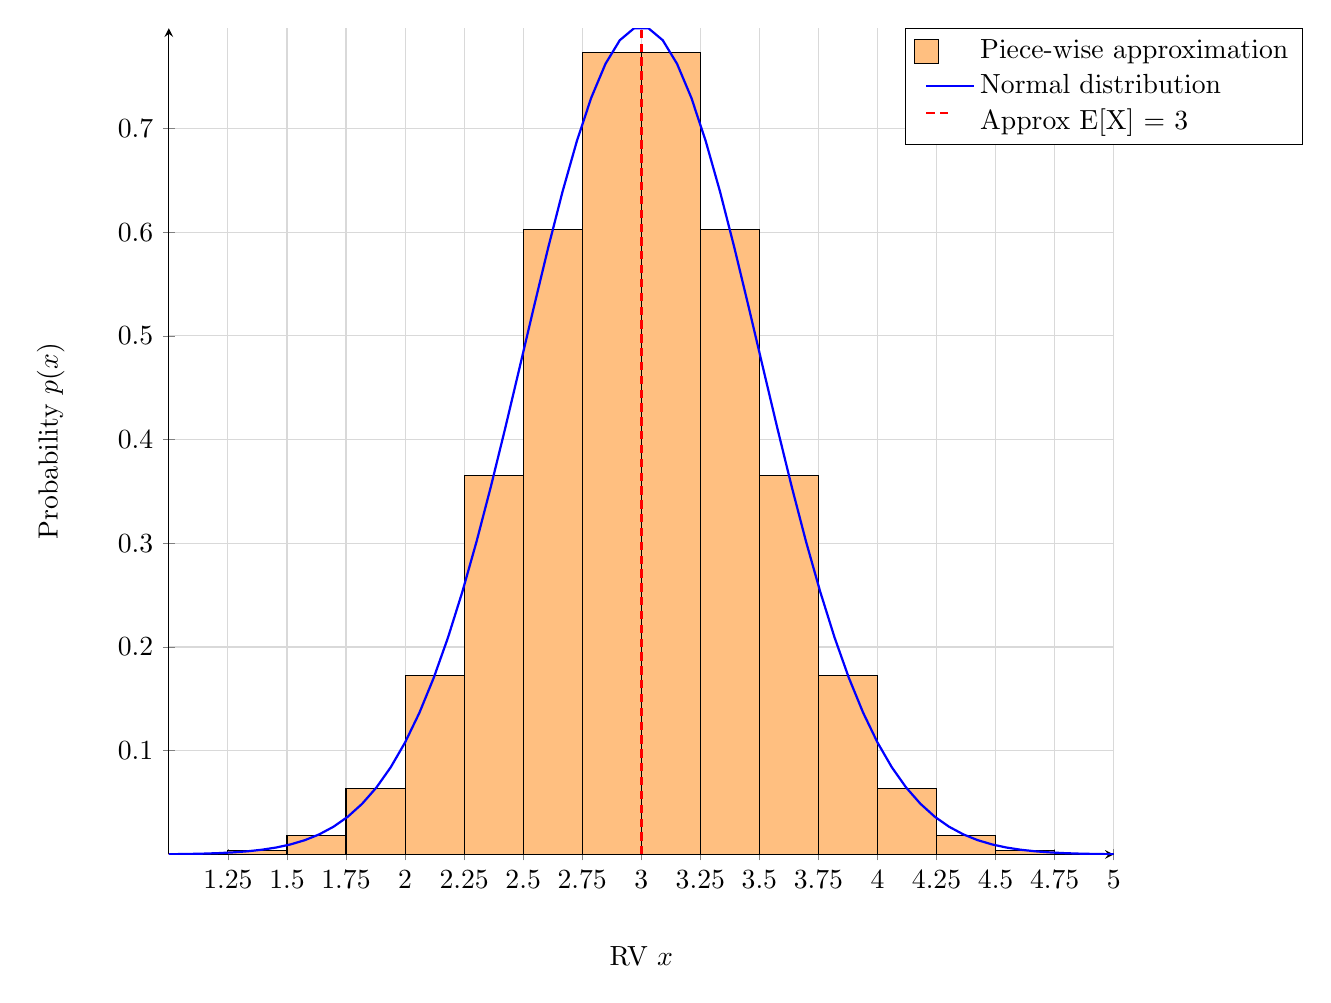
\begin{tikzpicture}
			\begin{axis}[
				domain=0:6,
				samples=100,
				axis lines=middle,
				xlabel={RV $x$},
				ylabel={Probability $p(x)$},
				xlabel style={
					at={(axis description cs:0.5,-0.1)}, anchor=north
				},
				ylabel style={
					rotate=90, % <-- rotation verticale
					at={(axis description cs:-0.1,0.5)}, anchor=south
				},
				width=14cm,
				x=3cm,
				grid=both,
				major grid style={gray!30},
				xtick={1,1.25,...,5},
				xmin=1,
				xmax=5,
				ymin=0,
				legend style={at={(1.2,1)}, anchor=north east},
				legend cell align=left,
				]
				
				% Barres
				\addplot[
				fill=orange!50,
				draw=black,
				ybar,
				bar width=0.75cm,
				legend image code/.code={
					\draw[fill=orange!50, draw=black] (-0.15cm,-0.15cm) rectangle (0.15cm,0.15cm);
				},
				] table[x=x, y=y, row sep=\\] {
					x y \\
					1.125 0.000705191365 \\
					1.375 0.004058096115 \\
					1.625 0.018187125 \\
					1.875 0.06347930367 \\
					2.125 0.1725546377 \\
					2.375 0.3652981708 \\
					2.625 0.6022748643 \\
					2.875 0.7733362336 \\
					3.125 0.7733362336 \\
					3.375 0.6022748643 \\
					3.625 0.3652981708 \\
					3.875 0.1725546377 \\
					4.125 0.06347930367 \\
					4.375 0.018187125 \\
					4.625 0.004058096115 \\
					4.875 0.000705191365 \\
				};
				
				\addlegendentry{Piece-wise approximation}
				
				% Courbe normale
				\def\mu{3}
				\def\sigma{0.5}
				
				\addplot[
				thick,
				blue,
				] {1/( \sigma * sqrt(2*pi)) * exp(-0.5*((x-\mu)/\sigma)^2)};
				\addlegendentry{Normal distribution}
				
				% Ligne verticale rouge
				\draw[densely dashed, very thick, red]
				(axis cs:3,0) -- (axis cs:3,1);
				
				% Pour la légende
				\addplot[
				red,
				densely dashed,
				thick,
				mark=none,
				legend image code/.code={
					\draw[red, densely dashed, thick] (0cm,0.1cm) -- (0.3cm,0.1cm);
				}
				] coordinates {(0,0) (1,0)};
				\addlegendentry{Approx E[X] = 3}
				
			\end{axis}
		\end{tikzpicture}
	\end{center}
	
\end{document}
